\chapter{Mining Economics: Hashprice, Efficiency, Breakeven}
\chaptermark{Mining Economics}
\label{ch:economics}

Part I ended with a market that pays loads to be flexible. Before this book can price that flexibility, it has to answer a more basic question: what does a mining machine actually earn, what does it spend, and where exactly is zero? Chapter~1 promised the full derivation of the breakeven arithmetic; this chapter delivers it, and everything after runs on it. One formula connects the mining industry's unit system (dollars per terahash-day) to the energy industry's (dollars per megawatt-hour). Once you can move between those two currencies, curtailment strategies, strike prices, and ancillary-service bids all become readable.

\section{What a Miner Sells}

A Bitcoin miner sells computation to a buyer that never negotiates. The Bitcoin network pays out a fixed daily pot: one block roughly every ten minutes, 144 blocks in an expected day, each currently carrying a \glossaryterm{block-subsidy}{block subsidy} of 3.125 newly created bitcoin, so 450 BTC per day plus whatever transaction fees users attached that day \autocite{Nakamoto2008}. % src: 144 x 3.125 = 450 BTC/day; subsidy since the April 2024 halving; fee share source in verify pass
No customer orders this computation, and producing more of it does not enlarge the pot. Every miner in the world competes for a slice of the same pot, and each miner's expected slice is simply its share of the network's total computational rate, the hashrate introduced in Chapter~1.

For an energy reader, one feature of this business deserves emphasis: revenue is set globally, cost is set locally. A miner in West Texas and a miner in Norway earn exactly the same revenue per terahash. They differ only in what they pay for electricity, and in how cleverly they buy it. That is why the rest of this book is about the cost side, and why the world's most sophisticated mining operations concentrate wherever electricity is cheap, volatile, or both.

The pot itself is on a schedule. Every 210,000 blocks, roughly every four years, the block subsidy halves: the event the industry calls the \glossaryterm{halving}{halving}. On April 20, 2024, at block 840,000, the subsidy dropped from 6.25 to 3.125 bitcoin; around April 2028 it will drop to 1.5625 \autocite{mempool840000,pan2024halving,braiins2024miningbasics}. % src: block 840,000 timestamp 2024-04-20 00:09:27 UTC (mempool.space); US-timezone outlets say Apr 19, UTC is the 20th; next halving at block 1,050,000, "spring of 2028" per Braiins Academy, hedged as "around April 2028"
Overnight, with no change in demand, machines, or electricity prices, every miner's revenue per unit of work falls by very nearly half. No other commodity producer wakes up to a calendar-scheduled halving of its output. Miners plan around it the way farmers plan around winter.

\section{Hashprice: One Number for the Revenue Side}

The industry compresses the entire revenue side into a single quote: \glossaryterm{hashprice}{hashprice}, the dollars a unit of hashrate earns per day \autocite{braiinsacademyhashprice}. % src: Braiins Academy Hashpower FAQ: hashvalue = theoretical mining income for 1 PH/s per day in BTC; hashprice = the same in fiat
This book quotes it in dollars per terahash-day (\$/TH/day), a terahash-day being one terahash per second sustained for a day, as a megawatt-hour is one megawatt for an hour; market convention also uses \$/PH/day, a thousand times larger. The definition is a division:
\[
\text{hashprice} = \frac{\text{network revenue per day (subsidy} + \text{fees)} \times \text{bitcoin price}}{\text{network hashrate}}
\]
The arithmetic is worth doing once by hand. In August 2026, with bitcoin near \$66{,}000 and the network at about 930~EH/s (930 million TH/s), the subsidy alone paid $450 \times 66{,}000 / 930{,}000{,}000 \approx \$0.032$ per terahash-day, Chapter~1's figure, and the published hashprice index sat within a few percent of that \autocite{BraiinsInsightsHashprice}. % src: ch1 anchors from the committed caches (BTC $66,180 and 930.2 EH/s, 7-day means to 2026-08-21, analysis/checks/ch1_network_energy.R); unrounded, 450 x 66,180 / 930.2M = $0.03202, the rounded inputs above $0.03194, both $0.032; index read $0.031-0.032 mid-Aug 2026 (Braiins Insights hashrate-value-history; cache analysis/data/hashprice_daily.csv)
Transaction fees add a small stream on top; through 2025 and 2026 they typically contributed about one percent of miner revenue or less \autocite{coinmetrics2025sotn304,CoinSharesMiningQ12026}. % src: Coin Metrics SOTN 304: fees 1.33% of total miner revenue Q1 2025; CoinShares Q1 2026 report: fees consistently below 1% of block rewards in Q4 2025, ~0.018 BTC/block

Three principal drivers shape hashprice. A rising bitcoin price pushes it up. A rising network hashrate pushes it down: more machines splitting the same pot means less for each. And the halving cuts the subsidy in half on schedule. Fees add noise, occasionally a spike. Figure~\ref{fig:hashprice-cycle} shows all three drivers acting on two and a half years of data.

\begin{figure}[h]
  \centering
  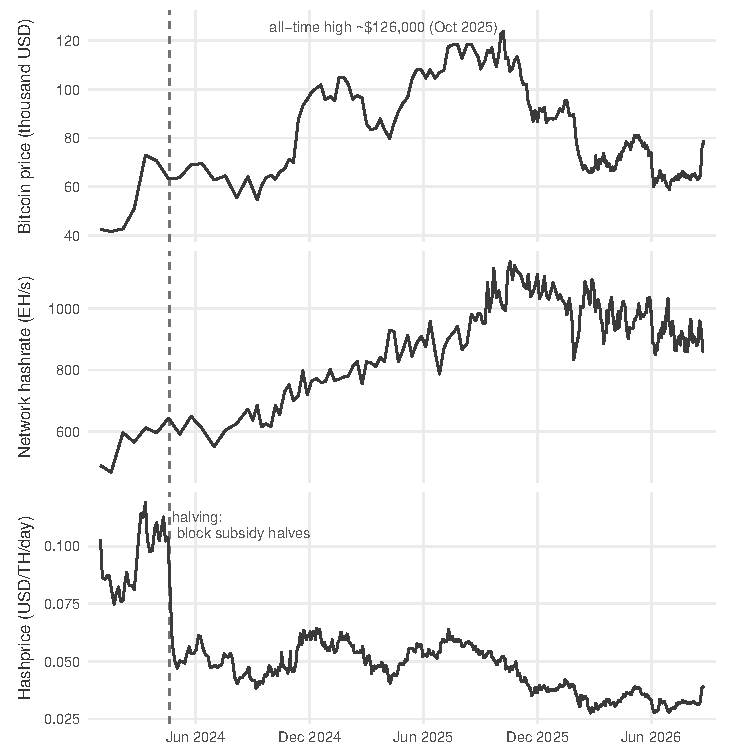
\includegraphics[width=\textwidth]{images/hashprice_cycle}
  \caption{
    The bitcoin price, the network hashrate, and hashprice, January 2024 to August 2026. Within a halving epoch, price and hashprice move together; across the April 2024 halving they decouple, because the halving cuts the newly issued bitcoin in half. The middle panel shows the network hashrate: every terahash that comes online dilutes the rest. Data: Braiins Insights \autocite{BraiinsInsightsHashprice}. % fig-src: analysis/figures/fig_ch4_hashprice_cycle.R (timeframes stitched to daily; Jan-Aug 2024 rests on the interpolated 5y frame)
  }
  \label{fig:hashprice-cycle}
\end{figure}

Does hashprice track the bitcoin price? Within a single halving epoch, yes, and increasingly tightly: the daily correlation between the two was 0.61 across 2025 and 0.90 in the 2026 bear leg. Across epochs, no: over the full window from January 2024 to mid-August 2026 the correlation is close to zero, because the halving sits in the middle of it. % src: Pearson r on stitched daily series, fig_ch4_hashprice_cycle.R console output 2026-08-24 (2025: 0.605; 2026 YTD: 0.901; full window: -0.08)
The bitcoin price rose by about two-thirds over that window; hashprice \emph{fell} by two-thirds. % src: BTC ~$42,600 (Jan 1, 2024) to ~$69,800 (Aug 12, 2026), +64%; hashprice $0.0921 to $0.0317, -66%; caches analysis/data/
Two structural forces produce that wedge. The halving cut the subsidy in half once, and relentless hashrate growth dilutes every survivor's share continuously. Hashprice rides the bitcoin cycle, but it rides it down an escalator.

The middle panel shows the machinery that connects the other two: a difficulty loop. A rising bitcoin price lifts hashprice at once. A high hashprice makes almost every machine on earth profitable, so more machines come online, and the network hashrate climbs: from roughly 490~EH/s in January 2024 to a peak above 1,100~EH/s in late 2025. % src: analysis/data/network_hashrate_daily.csv, the daily series the middle panel plots; analysis/checks/ch1_hashrate_peak.R console: 490.0 EH/s on 2024-01-01, daily max 1,151.5 EH/s on 2025-10-18, 7-day-mean peak 1,132.7 EH/s in the week to 2025-10-20 (fig_ch4_hashprice_cycle.R's console prints the same daily points rounded, 490 and 1151 EH/s)
Every new terahash raises the difficulty and dilutes each incumbent's share, which pushes hashprice back down. That is why the hashprice peaks of the 2024--2025 bull market kept coming in lower even as the bitcoin price kept setting records: each rally paid for the machines that diluted the next one. In 2026 the difficulty loop ran in reverse: hashprice fell below the breakeven of the fleet's weakest machines, machines switched off, and the hashrate in the middle panel rolls over, giving back a fifth to a quarter of its peak. % src: analysis/checks/ch1_hashrate_peak.R console: on 7-day means of analysis/data/network_hashrate_daily.csv, 1,132.7 EH/s (week to 2025-10-20) to 906.6 EH/s (week to 2026-08-24, the panel's last) is 20.0% given back, to 930.2 EH/s (week to 2026-08-21, ch1's anchor) 17.9%; on the daily points the panel plots, 25.4% (1,151.5 on 2025-10-18 to 859.1 on 2026-08-24; fig_ch4_hashprice_cycle.R's console: max 1151, 859 on 2026-08-24); ch1, ch4 and the glossary all date the peak to late 2025
Section~\ref{sec:sensitivity} shows what closes the difficulty loop at the level of a single machine.

The short run belongs to the bitcoin price, though, and it can move fast. In the week this chapter was drafted, a bitcoin rally of roughly a quarter lifted hashprice from \$0.031 to \$0.039 per terahash-day in eight days, tracking the price move almost one for one, because the difficulty happened to sit still the whole time. % src: stitched daily caches (analysis/data/): hashprice 0.0312 (Aug 16, 2026) to 0.0392 (Aug 24) = +25.6%; BTC 63,173 to 79,109 = +25.2%; difficulty 126.23T (Aug 6) to 125.81T (Aug 24), -0.3% (Braiins Insights difficulty series)
What that eight-tenths-of-a-cent move did to individual machines is the subject of the rest of this chapter.

\section{Efficiency: The Machine's Exchange Rate}

Hashprice prices computation. Electricity markets price energy. The bridge between them is the machine itself, and specifically the specification Chapter~1 called the most important one: efficiency, in joules per terahash (J/TH), the energy a machine spends to perform a unit of work. Efficiency is the exchange rate between the two currencies: it converts revenue per terahash into revenue per megawatt-hour, the number an energy trader actually wants.

The conversion deserves one careful derivation, because the book uses it constantly. A megawatt-hour is $3.6 \times 10^9$ joules. A machine with efficiency $e$ joules per terahash therefore performs $3.6 \times 10^9 / e$ terahashes per megawatt-hour consumed. Hashprice pays per terahash-day, which is $86{,}400$ terahashes, so one megawatt-hour earns:
\[
\text{revenue per MWh} = \text{hashprice} \times \frac{3.6 \times 10^9}{e \times 86{,}400} = \frac{41{,}667 \times \text{hashprice}}{e}
\]
with hashprice in \$/TH/day and $e$ in J/TH. % src: identity; constant 3.6e9/86,400 = 41,666.7; same form as the PAPO algorithm's revenue equation (papo-model-algo/PAPO_ALGORITHM.md)
The constant 41,667 is worth memorizing; it is the book's Rosetta Stone, and it will reappear in every Part III chapter.

Two machines carry the argument from here, chosen because together they bracket the working fleet. The \glossaryterm{antminer-s19j-pro}{Antminer S19j~Pro} is a 2021-vintage workhorse that still populates mining farms in large numbers: 104~TH/s at 3,068~W, which is 29.5~J/TH \autocite{bitmain2021s19jpro}. % src: Bitmain S19j Pro Specifications, 104T variant: 3068 W +/-5%, 29.5 J/TH (all variants); article created Jun 2021
The \glossaryterm{antminer-s21-xp}{Antminer S21~XP} is the 2024 flagship of the same manufacturer: 270~TH/s at 3,645~W, which is 13.5~J/TH \autocite{bitmain2024s21xp}. % src: Bitmain S21 XP Specifications: 3645 W on wall @25C +/-5% (4,000 W is the PSU requirement, not draw; some listings' 3,900 W is not Bitmain's rating); 13.5 J/TH; article created Jul 2024
The newer machine is not faster in any way that matters to this chapter; it is \emph{cheaper to feed}. At the 2025 average hashprice of about \$0.051 per terahash-day, the exchange-rate formula says the S19j~Pro turned each megawatt-hour into roughly \$72 of bitcoin, and the S21~XP turned the same megawatt-hour into \$157. % src: 41,666.7 x 0.0507 / 29.5 = 71.6; / 13.5 = 156.5; 2025 mean hashprice 0.0507 from analysis/data/hashprice_daily.csv
Under the same market conditions, the more efficient machine earns more than twice as much revenue per megawatt-hour.

\section{Breakeven: The Number That Runs the Business}

Set revenue per megawatt-hour equal to the price of a megawatt-hour and you get the number every mining operator knows by heart, the \glossaryterm{breakeven-price}{breakeven price}:
\[
P_{\text{breakeven}} = \frac{41{,}667 \times \text{hashprice}}{e}
\]
Read in this direction, it answers the operator's daily question: given today's hashprice, what electricity price can my machines afford? Solved for hashprice instead,
\[
\text{hashprice}_{\text{breakeven}} = \frac{e \times P}{41{,}667},
\]
it answers the investor's question: given my power contract, what hashprice keeps my machines alive? The two forms are one equation, and readers from either industry will need both.

To be precise, this breakeven is an \emph{operating} threshold. It compares revenue against electricity alone, and electricity is the dominant but not the only cost of running a mine; it ignores the capital cost of the machine, hosting, cooling, and staff. A machine below its operating breakeven loses money on every hour it runs and should stop immediately. A machine above it contributes margin, whether or not the site as a whole ever recovers its investment. Grid economics has the same distinction: this is the shutdown point, not the entry decision.

\section{Two Machines, One Hashprice}
\label{sec:sensitivity}

Now freeze everything except hashprice. Fix each machine at its stock operating point, so efficiency is a constant rather than a curve (the curve is Chapter~5's subject). Fix the electricity price at \$42.18 per megawatt-hour, the average 15-minute real-time settlement point price in LZ\_WEST across calendar 2025, the zone where this book's miners live; the market monitor's own accounting puts the zone's load-weighted average at \$41.59, the highest of any ERCOT zone that year \autocite{ercot2026rtm,potomac2026somercot}. % src: $42.18 = mean of all 35,040 15-min settlement prices, LZ_WEST 2025, from ERCOT MIS report 13061 (analysis/data/ercot_rtm15_spp_loadzones_2021on.csv.gz, built by analysis/data/fetch_ercot_rtm15_spp_history.py; console of analysis/figures/fig_ch6_strike.R). Supersedes the $42.22 of the older ingest cache, which dropped the nine spring-forward intervals; author confirmed $42.18 on 2026-09-04. The ERCOT-direct re-derivation pin is RESOLVED (2026-08-28). Cross-checks: 5-min series mean $41.79 (lz_west_rt_annual_means.csv); SOM load-weighted ex-adders $41.59 + ~$0.43 adders ~ $42.0. RT settlement is the book's reference price (author decision 2026-08-24)
A real ERCOT miner faces a different price every quarter-hour and that variance is where Part III finds its money; the flat average is deliberately artificial, a laboratory stand-in that isolates one variable. What remains is a clean experiment: sweep hashprice, watch two machines respond.

\begin{figure}[h]
  \centering
  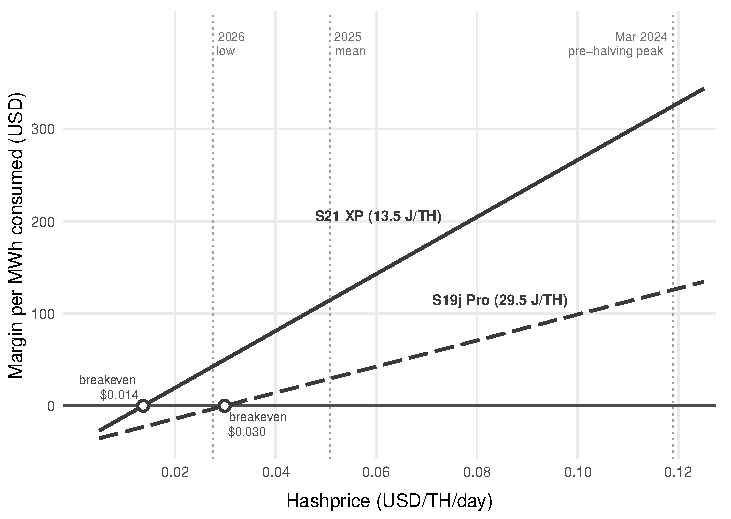
\includegraphics[width=\textwidth]{images/miner_sensitivity}
  \caption{
    Margin per megawatt-hour consumed as a function of hashprice, with efficiency fixed at stock and electricity fixed at the 2025 mean LZ\_WEST real-time settlement point price of \$42.18/MWh. Dotted verticals mark where hashprice actually traded: the March 2024 pre-halving peak, the 2025 mean, and the 2026 low. The S21~XP breaks even at \$0.014 per terahash-day, below anything the market has recorded; the S19j~Pro breaks even at \$0.030, a line the market crossed in 2026. % fig-src: analysis/figures/fig_ch4_sensitivity.R
  }
  \label{fig:miner-sensitivity}
\end{figure}

Figure~\ref{fig:miner-sensitivity} shows the result, and Table~\ref{tab:miner-sensitivity} gives the exact numbers at three hashprice levels the market actually visited: the 2026 low, the 2025 average, and the March 2024 pre-halving peak.

\begin{table}[h]
  \centering
  \small
  \begin{tabular}{lrr}
    \hline
    & \textbf{S19j Pro} & \textbf{S21 XP} \\
    \hline
    Hashrate & 104 TH/s & 270 TH/s \\
    Power draw (stock) & 3,068 W & 3,645 W \\
    Efficiency & 29.5 J/TH & 13.5 J/TH \\
    Electricity per day & 73.6 kWh & 87.5 kWh \\
    Electricity cost per day (at \$42.18/MWh) & \$3.11 & \$3.69 \\
    Breakeven hashprice & \$0.030 & \$0.014 \\
    \hline
    Profit per day at 2026 low (\$0.028) & $-$\$0.24 & +\$3.75 \\
    Profit per day at 2025 mean (\$0.051) & +\$2.18 & +\$10.02 \\
    Profit per day at Mar 2024 peak (\$0.119) & +\$9.26 & +\$28.42 \\
    \hline
  \end{tabular}
  \caption{Daily economics of the two machines at three hashprice levels. Stock specifications; electricity fixed at the 2025 mean LZ\_WEST real-time price. Profit here is revenue minus electricity only.} % src: computed in analysis/figures/fig_ch4_sensitivity.R (console output; landmarks read from the cache: 2024 max $0.11891 on 2024-03-13, 2025 mean $0.05082, 2026 min $0.02757 on 2026-02-24); hashprice landmarks from analysis/data/hashprice_daily.csv; RT mean from analysis/data/lz_west_rt_annual_means.csv
  \label{tab:miner-sensitivity}
\end{table}

Read the table bottom-up, from boom to bust. At the pre-halving peak, both machines printed money and the S19j~Pro's inefficiency did not threaten its margin; this is the regime in which nobody curtails and efficiency debates feel academic. At the 2025 average, the S19j~Pro still cleared about \$2 a day, a real but thinning margin. At the 2026 low, the two machines were no longer in the same business: the S21~XP still earned \$3.75 a day, while the S19j~Pro lost money every hour it ran.

The asymmetry has a name in any commodity industry: operating leverage. On the eve of the August 2026 rally, the S19j~Pro was spending 96 cents of every revenue dollar on electricity; the S21~XP was spending about 44. % src: at HP $0.0312 (Aug 16, 2026, pre-rally trough): S19j cost/rev = 3.11/3.24 = 0.96; S21 XP = 3.69/8.42 = 0.44; cost/day = W x 24h x $42.18/MWh: S19j 73.6 kWh -> $3.11, S21 87.5 kWh -> $3.69; rev/day = HP x TH: S19j 104 x 0.0312 = $3.24, S21 270 x 0.0312 = $8.42
A ten percent move in hashprice barely registers at the efficient machine and doubles or erases the inefficient one's entire margin. The week-long rally from \$0.031 to \$0.039 took the S19j~Pro from earning 14 cents a day to earning nearly a dollar, a sevenfold change, while the S21~XP improved by a comfortable but unremarkable half. % src: S19j: 104 x 0.0312 - 3.11 = +$0.14; 104 x 0.0392 - 3.11 = +$0.97; S21 XP: +$4.73 to +$6.89, +46%
Efficiency raises profits and reduces the machine's exposure to hashprice.

Here is the machine-level view of the difficulty loop in Figure~\ref{fig:hashprice-cycle}, and Chapter~2 already showed its fastest version in action. When hashprice falls below the breakeven of the fleet's marginal machines, those machines shut down; the network hashrate falls; the difficulty adjustment pays every surviving machine more; hashprice climbs back toward the new marginal breakeven. The network continuously reprices itself so that the worst machine still running earns roughly zero. % src: difficulty adjustment mechanism, Nakamoto2008; observed post-Fern: -11.16% adjustment then +14.73% recovery (ch2, BraiinsInsights)
That is why the S19j~Pro generation is not simply dead: every time enough of its cohort switches off, the survivors get a raise. The fleet lives on the breakeven line by construction, which means the marginal machine, wherever it is, mines for nearly nothing. Its only remaining edge is the price it pays for power.

\section{What This Means on a Grid}

Flip the breakeven formula one last time and it stops being an investor's metric and becomes an operating instruction. At any moment, a machine's breakeven price is the electricity price above which it is worth more switched off than on. At the 2025 average hashprice, the S19j~Pro's breakeven was about \$72 per megawatt-hour, a level LZ\_WEST real-time prices crossed routinely; the S21~XP's was about \$157, crossed far more rarely. % src: 41,666.7 x 0.0507 / 29.5 = 71.6; / 13.5 = 156.5; LZ_WEST exceedances quantified in ch6
In a market that reprices every few minutes (Chapter~3), that threshold is not a diagnosis. It is a tripwire: the moment the real-time price crosses it, the machine should stop, and the response can be automatic. The afternoon's day-ahead preview is still useful for flagging which hours look dangerous in advance, but the trigger itself is the real-time price. % src: reframed from "schedule" to reactive trigger per the ch6 RTM-strike decision (author, 2026-08-24)

The efficient machine survives expensive hours that kill the inefficient one, so efficiency buys \emph{endurance}. But the inefficient machine crosses its threshold more often, so it curtails more, and in programs that pay for flexibility it has more flexibility to sell. The S21~XP earns its money by running; the S19j~Pro increasingly earns its keep by knowing when to stop. Chapter~5 puts the two behaviors on one curve, because modern firmware lets a single machine slide between them; Chapter~6 turns the threshold into a strike price on the real-time market (a backstop that steps the machine out of price spikes) and prices the hours themselves. % src: ch6 strike analysis = RTM-reactive spike-avoidance backstop (author decision 2026-08-24; chapter 5's backstop implements it, analysis/ch5-backtest/papo_sim.py), NOT a day-ahead-scheduled strike

This chapter fixed efficiency and the power price to isolate hashprice. Every later chapter relaxes one of those clamps. Parts II and III look for the money in the variables this chapter held still.
